\documentclass{standalone}
\usepackage{pgfplots}
\begin{document}
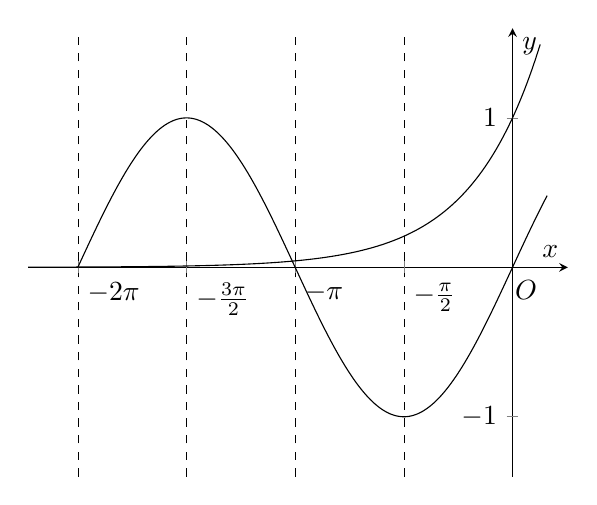
\begin{tikzpicture}
\begin{axis}
[
ymin=-1.4,ymax=1.6,
xmin=-7,xmax=0.8,
xtick=\empty,
ytick=\empty,
extra x ticks={-6.28319, -4.71239, -3.14159, -1.5708},
extra x tick labels={$-2\pi$, $-\frac{3\pi}{2}$, $-\pi$, $-\frac{\pi}{2}$},
extra y ticks={-1, 1},
extra y tick labels={$-1$, $1$},
every extra x tick/.style={
    xticklabel style={anchor=north west},
    grid=major,
    major grid style={very thin,dashed,black}
},
axis lines = center,
xlabel=$x$,ylabel=$y$,
samples=200,
]
\addplot [black, domain=-6.28319:0.5] {sin(deg(x))};
\addplot [black, domain=-7:0.4] {exp(x)};
\node at (axis cs:0.195, -0.15) {$O$} ;
\end{axis}
\end{tikzpicture}
\end{document}
